\clearpage
\subsection{Compact boson, small intervals}
\label{sec:pair-small_boson}
\begin{figure}[!htbp]\centering
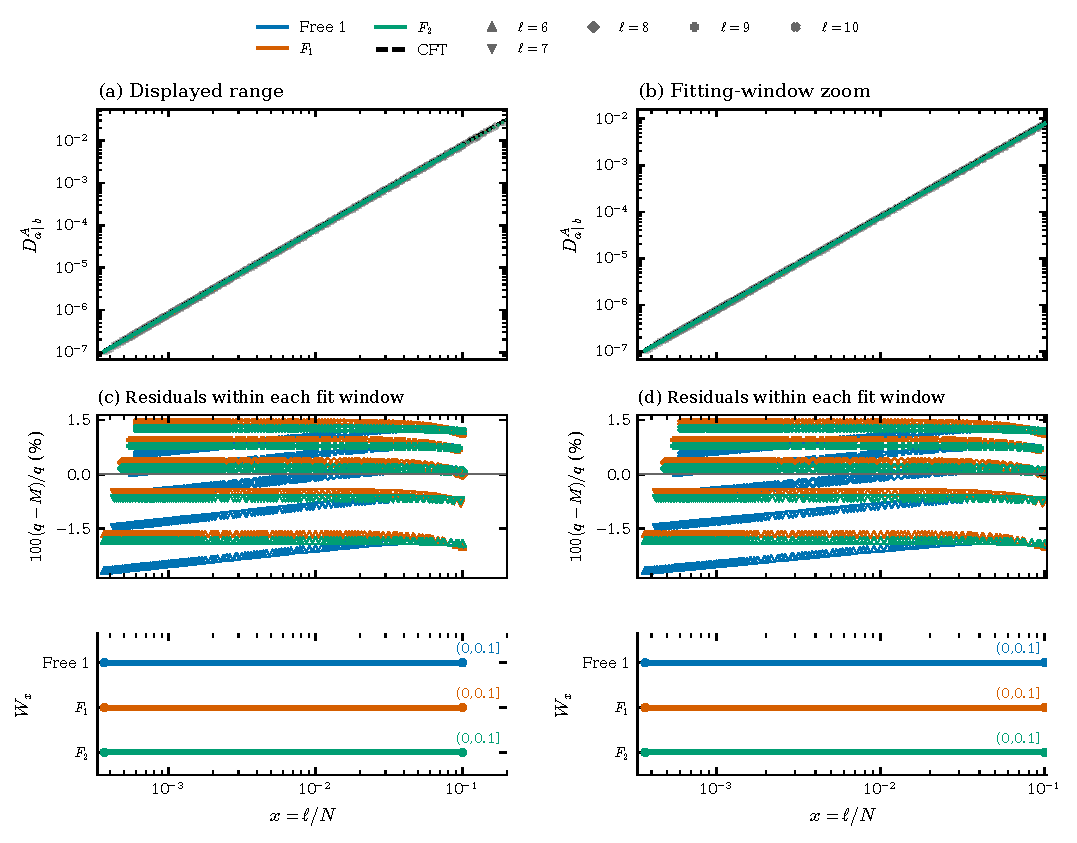
\includegraphics[width=.94\linewidth]{../figs/pair_small_boson_00_ss.pdf}\par\smallskip
\begingroup\scriptsize\setlength{\tabcolsep}{4pt}
\begin{tabular}{lllrrrrr}\toprule
Set & Model & $W_z$ & $m$ & $c_0$ & $r^{(0)}$ & $c_1$ & $r^{(1)}$\\\midrule
Both & Free 1 & $(0,0.1]$ & 598 & 0.77501 & 1.998159 & --- & ---\\
Both & $F_1$ & $(0,0.1]$ & 598 & 0.77866 & 2 & --- & ---\\
Both & $F_2$ & $(0,0.1]$ & 598 & 0.77996 & 2 & -0.1917 & 4\\
\midrule
Both & CFT & --- & --- & 0.82247 & 2 & --- & ---\\
\bottomrule\end{tabular}
\endgroup
\caption{Compact boson, small intervals, $00\mid ss$, at $p=1/2$, $\ell=6,\ldots,10$, and the complete size grid in Eq.~\eqref{eq:extended-grid}. Here $z=x$ and $q=D^A$. Left: all computed data through $z=0.20$; right: a zoom into the common fitting window. Both columns show the same Free 1, $F_1$, and $F_2$ fits. All six directions of this CFT and interval type use the same window. Gray markers denote the data. Colored solid segments lie inside each model\textquotesingle s fitting interval; dotted segments are extrapolations. Black dashed is the supplied CFT series. The observable axes are logarithmic and span the measured data; nonpositive predictions cannot appear there and out-of-range extrapolations leave the panel. Residual ordinates are linear and show $100(q-M)/q$ only on each model\textquotesingle s fitted observations. Bars give the exact fitting intervals. The parameter block follows Eq.~\eqref{eq:fit}, with $c_0,c_1$ multiplying $z^{r^{(0)}},z^{r^{(1)}}$; all coefficients include powers of $\pi$. A dash means an absent fitted term, or no fitting window for CFT. Values shown are rounded; curves use full precision.}
\label{fig:pair-small_boson-00-ss}
\end{figure}
\begin{figure}[!htbp]\centering
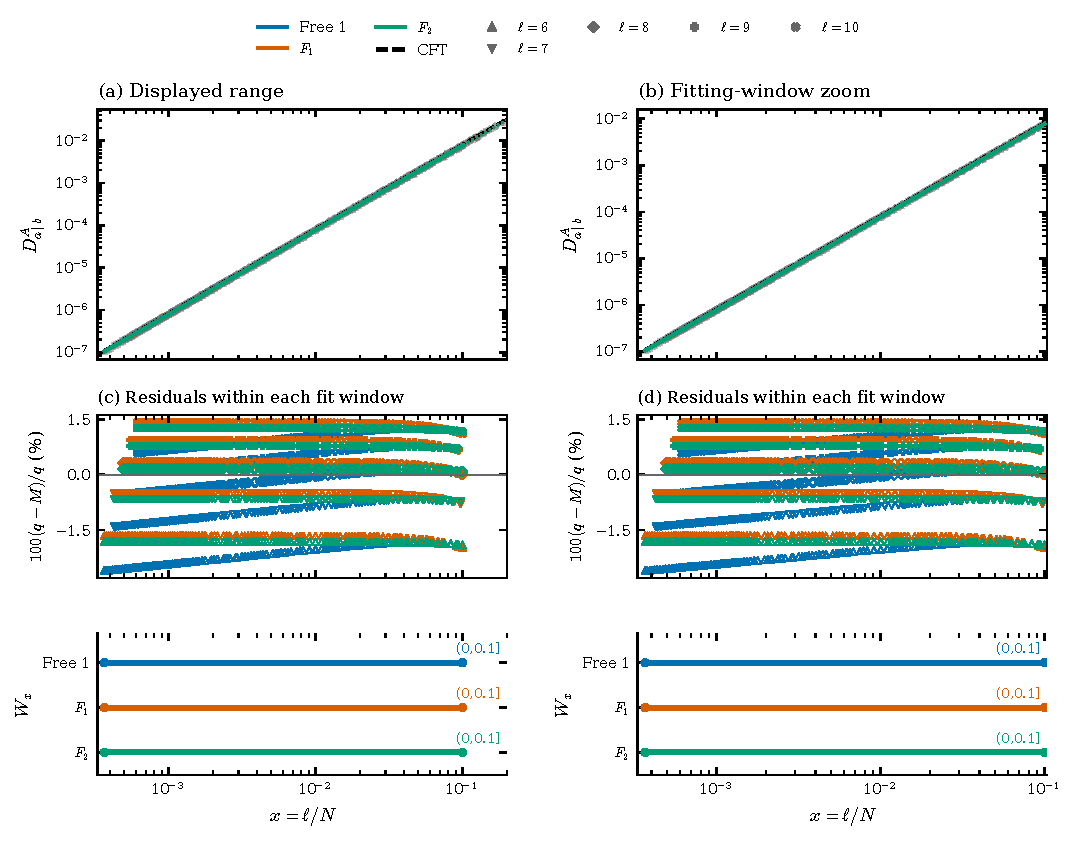
\includegraphics[width=.94\linewidth]{../figs/pair_small_boson_ss_00.pdf}\par\smallskip
\begingroup\scriptsize\setlength{\tabcolsep}{4pt}
\begin{tabular}{lllrrrrr}\toprule
Set & Model & $W_z$ & $m$ & $c_0$ & $r^{(0)}$ & $c_1$ & $r^{(1)}$\\\midrule
Both & Free 1 & $(0,0.1]$ & 598 & 0.77529 & 1.9982698 & --- & ---\\
Both & $F_1$ & $(0,0.1]$ & 598 & 0.77871 & 2 & --- & ---\\
Both & $F_2$ & $(0,0.1]$ & 598 & 0.77995 & 2 & -0.18219 & 4\\
\midrule
Both & CFT & --- & --- & 0.82247 & 2 & --- & ---\\
\bottomrule\end{tabular}
\endgroup
\caption{Compact boson, small intervals, $ss\mid 00$, at $p=1/2$, $\ell=6,\ldots,10$, and the complete size grid in Eq.~\eqref{eq:extended-grid}. Here $z=x$ and $q=D^A$. Left: all computed data through $z=0.20$; right: a zoom into the common fitting window. Both columns show the same Free 1, $F_1$, and $F_2$ fits. All six directions of this CFT and interval type use the same window. Gray markers denote the data. Colored solid segments lie inside each model\textquotesingle s fitting interval; dotted segments are extrapolations. Black dashed is the supplied CFT series. The observable axes are logarithmic and span the measured data; nonpositive predictions cannot appear there and out-of-range extrapolations leave the panel. Residual ordinates are linear and show $100(q-M)/q$ only on each model\textquotesingle s fitted observations. Bars give the exact fitting intervals. The parameter block follows Eq.~\eqref{eq:fit}, with $c_0,c_1$ multiplying $z^{r^{(0)}},z^{r^{(1)}}$; all coefficients include powers of $\pi$. A dash means an absent fitted term, or no fitting window for CFT. Values shown are rounded; curves use full precision.}
\label{fig:pair-small_boson-ss-00}
\end{figure}
\begin{figure}[!htbp]\centering
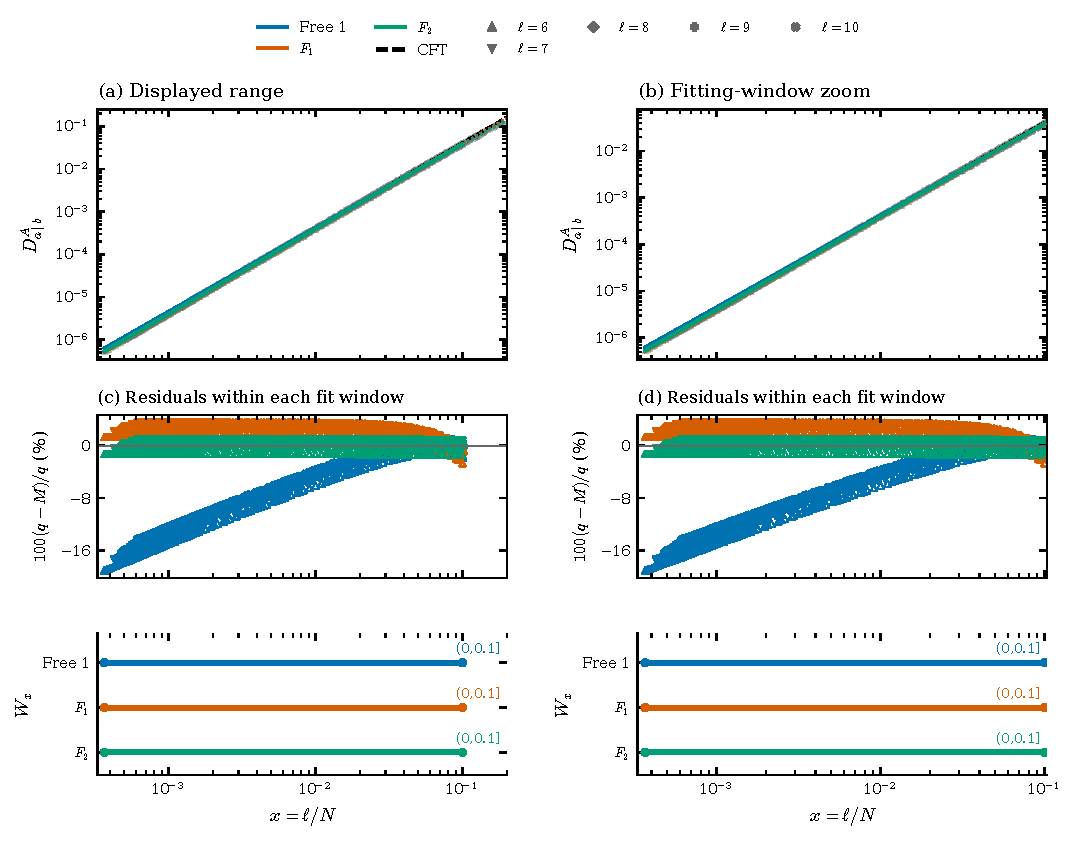
\includegraphics[width=.94\linewidth]{../figs/pair_small_boson_00_3s_s.pdf}\par\smallskip
\begingroup\scriptsize\setlength{\tabcolsep}{4pt}
\begin{tabular}{lllrrrrr}\toprule
Set & Model & $W_z$ & $m$ & $c_0$ & $r^{(0)}$ & $c_1$ & $r^{(1)}$\\\midrule
Both & Free 1 & $(0,0.1]$ & 598 & 3.5315 & 1.9648776 & --- & ---\\
Both & $F_1$ & $(0,0.1]$ & 598 & 3.8623 & 2 & --- & ---\\
Both & $F_2$ & $(0,0.1]$ & 598 & 3.964 & 2 & -15.02 & 4\\
\midrule
Both & CFT & --- & --- & 4.1123 & 2 & --- & ---\\
\bottomrule\end{tabular}
\endgroup
\caption{Compact boson, small intervals, $00\mid 3s,s$, at $p=1/2$, $\ell=6,\ldots,10$, and the complete size grid in Eq.~\eqref{eq:extended-grid}. Here $z=x$ and $q=D^A$. Left: all computed data through $z=0.20$; right: a zoom into the common fitting window. Both columns show the same Free 1, $F_1$, and $F_2$ fits. All six directions of this CFT and interval type use the same window. Gray markers denote the data. Colored solid segments lie inside each model\textquotesingle s fitting interval; dotted segments are extrapolations. Black dashed is the supplied CFT series. The observable axes are logarithmic and span the measured data; nonpositive predictions cannot appear there and out-of-range extrapolations leave the panel. Residual ordinates are linear and show $100(q-M)/q$ only on each model\textquotesingle s fitted observations. Bars give the exact fitting intervals. The parameter block follows Eq.~\eqref{eq:fit}, with $c_0,c_1$ multiplying $z^{r^{(0)}},z^{r^{(1)}}$; all coefficients include powers of $\pi$. A dash means an absent fitted term, or no fitting window for CFT. Values shown are rounded; curves use full precision.}
\label{fig:pair-small_boson-00-3s_s}
\end{figure}
\begin{figure}[!htbp]\centering
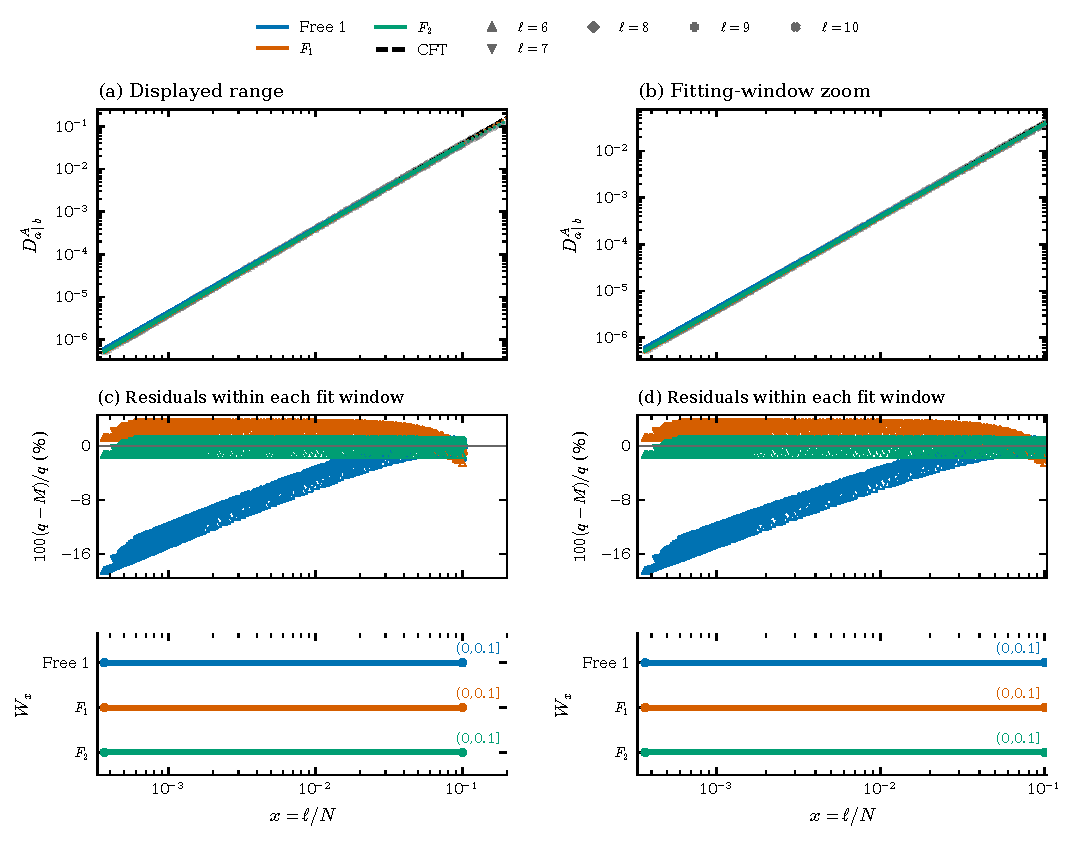
\includegraphics[width=.94\linewidth]{../figs/pair_small_boson_3s_s_00.pdf}\par\smallskip
\begingroup\scriptsize\setlength{\tabcolsep}{4pt}
\begin{tabular}{lllrrrrr}\toprule
Set & Model & $W_z$ & $m$ & $c_0$ & $r^{(0)}$ & $c_1$ & $r^{(1)}$\\\midrule
Both & Free 1 & $(0,0.1]$ & 598 & 3.545 & 1.9660249 & --- & ---\\
Both & $F_1$ & $(0,0.1]$ & 598 & 3.8657 & 2 & --- & ---\\
Both & $F_2$ & $(0,0.1]$ & 598 & 3.9643 & 2 & -14.541 & 4\\
\midrule
Both & CFT & --- & --- & 4.1123 & 2 & --- & ---\\
\bottomrule\end{tabular}
\endgroup
\caption{Compact boson, small intervals, $3s,s\mid 00$, at $p=1/2$, $\ell=6,\ldots,10$, and the complete size grid in Eq.~\eqref{eq:extended-grid}. Here $z=x$ and $q=D^A$. Left: all computed data through $z=0.20$; right: a zoom into the common fitting window. Both columns show the same Free 1, $F_1$, and $F_2$ fits. All six directions of this CFT and interval type use the same window. Gray markers denote the data. Colored solid segments lie inside each model\textquotesingle s fitting interval; dotted segments are extrapolations. Black dashed is the supplied CFT series. The observable axes are logarithmic and span the measured data; nonpositive predictions cannot appear there and out-of-range extrapolations leave the panel. Residual ordinates are linear and show $100(q-M)/q$ only on each model\textquotesingle s fitted observations. Bars give the exact fitting intervals. The parameter block follows Eq.~\eqref{eq:fit}, with $c_0,c_1$ multiplying $z^{r^{(0)}},z^{r^{(1)}}$; all coefficients include powers of $\pi$. A dash means an absent fitted term, or no fitting window for CFT. Values shown are rounded; curves use full precision.}
\label{fig:pair-small_boson-3s_s-00}
\end{figure}
\begin{figure}[!htbp]\centering
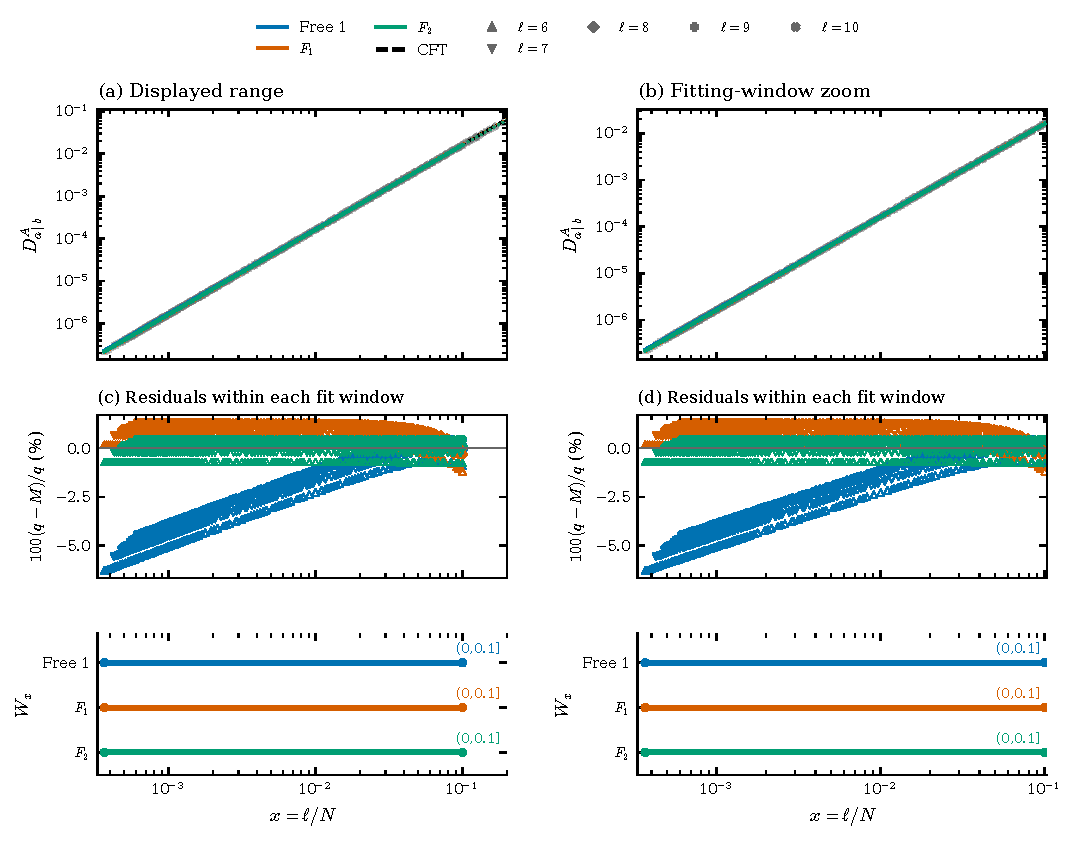
\includegraphics[width=.94\linewidth]{../figs/pair_small_boson_ss_3s_s.pdf}\par\smallskip
\begingroup\scriptsize\setlength{\tabcolsep}{4pt}
\begin{tabular}{lllrrrrr}\toprule
Set & Model & $W_z$ & $m$ & $c_0$ & $r^{(0)}$ & $c_1$ & $r^{(1)}$\\\midrule
Both & Free 1 & $(0,0.1]$ & 598 & 1.5661 & 1.9883068 & --- & ---\\
Both & $F_1$ & $(0,0.1]$ & 598 & 1.6134 & 2 & --- & ---\\
Both & $F_2$ & $(0,0.1]$ & 598 & 1.6276 & 2 & -2.0896 & 4\\
\midrule
Both & CFT & --- & --- & 1.6449 & 2 & --- & ---\\
\bottomrule\end{tabular}
\endgroup
\caption{Compact boson, small intervals, $ss\mid 3s,s$, at $p=1/2$, $\ell=6,\ldots,10$, and the complete size grid in Eq.~\eqref{eq:extended-grid}. Here $z=x$ and $q=D^A$. Left: all computed data through $z=0.20$; right: a zoom into the common fitting window. Both columns show the same Free 1, $F_1$, and $F_2$ fits. All six directions of this CFT and interval type use the same window. Gray markers denote the data. Colored solid segments lie inside each model\textquotesingle s fitting interval; dotted segments are extrapolations. Black dashed is the supplied CFT series. The observable axes are logarithmic and span the measured data; nonpositive predictions cannot appear there and out-of-range extrapolations leave the panel. Residual ordinates are linear and show $100(q-M)/q$ only on each model\textquotesingle s fitted observations. Bars give the exact fitting intervals. The parameter block follows Eq.~\eqref{eq:fit}, with $c_0,c_1$ multiplying $z^{r^{(0)}},z^{r^{(1)}}$; all coefficients include powers of $\pi$. A dash means an absent fitted term, or no fitting window for CFT. Values shown are rounded; curves use full precision.}
\label{fig:pair-small_boson-ss-3s_s}
\end{figure}
\begin{figure}[!htbp]\centering
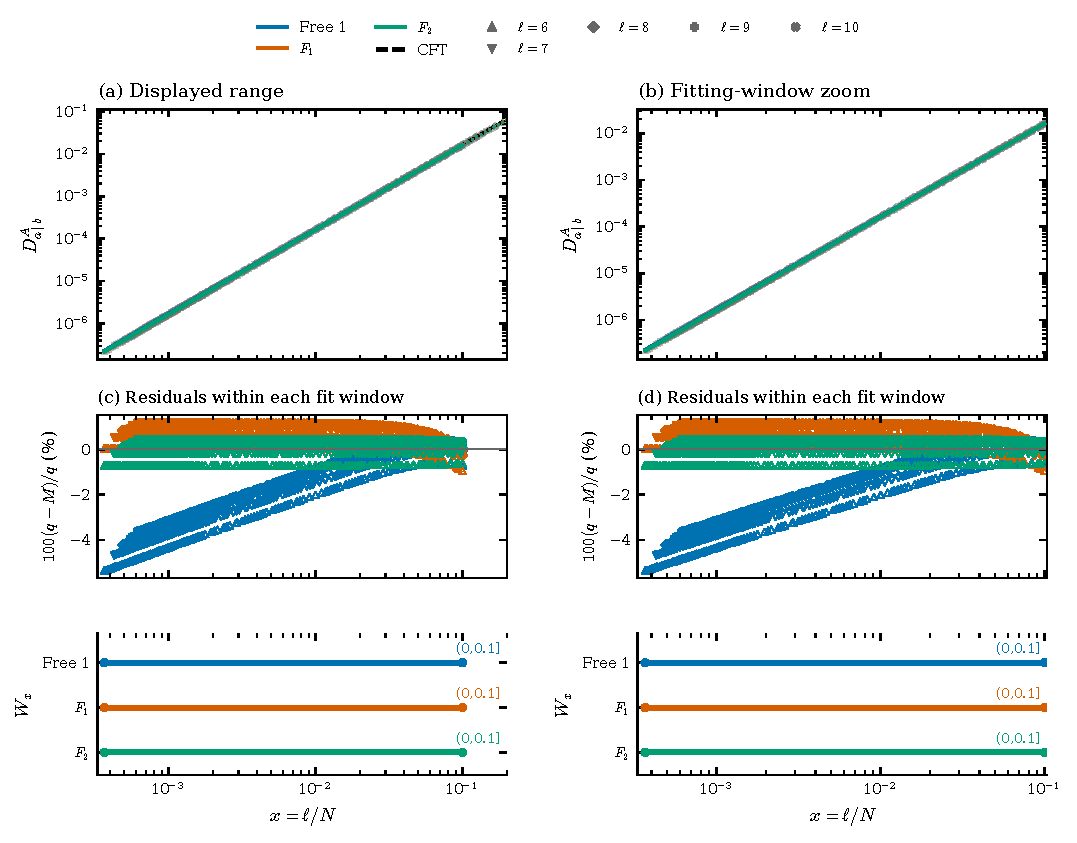
\includegraphics[width=.94\linewidth]{../figs/pair_small_boson_3s_s_ss.pdf}\par\smallskip
\begingroup\scriptsize\setlength{\tabcolsep}{4pt}
\begin{tabular}{lllrrrrr}\toprule
Set & Model & $W_z$ & $m$ & $c_0$ & $r^{(0)}$ & $c_1$ & $r^{(1)}$\\\midrule
Both & Free 1 & $(0,0.1]$ & 598 & 1.576 & 1.9902202 & --- & ---\\
Both & $F_1$ & $(0,0.1]$ & 598 & 1.6157 & 2 & --- & ---\\
Both & $F_2$ & $(0,0.1]$ & 598 & 1.6276 & 2 & -1.7507 & 4\\
\midrule
Both & CFT & --- & --- & 1.6449 & 2 & --- & ---\\
\bottomrule\end{tabular}
\endgroup
\caption{Compact boson, small intervals, $3s,s\mid ss$, at $p=1/2$, $\ell=6,\ldots,10$, and the complete size grid in Eq.~\eqref{eq:extended-grid}. Here $z=x$ and $q=D^A$. Left: all computed data through $z=0.20$; right: a zoom into the common fitting window. Both columns show the same Free 1, $F_1$, and $F_2$ fits. All six directions of this CFT and interval type use the same window. Gray markers denote the data. Colored solid segments lie inside each model\textquotesingle s fitting interval; dotted segments are extrapolations. Black dashed is the supplied CFT series. The observable axes are logarithmic and span the measured data; nonpositive predictions cannot appear there and out-of-range extrapolations leave the panel. Residual ordinates are linear and show $100(q-M)/q$ only on each model\textquotesingle s fitted observations. Bars give the exact fitting intervals. The parameter block follows Eq.~\eqref{eq:fit}, with $c_0,c_1$ multiplying $z^{r^{(0)}},z^{r^{(1)}}$; all coefficients include powers of $\pi$. A dash means an absent fitted term, or no fitting window for CFT. Values shown are rounded; curves use full precision.}
\label{fig:pair-small_boson-3s_s-ss}
\end{figure}
